\documentclass[paper=a4, fontsize=11pt]{scrartcl} % A4 paper and 11pt font size
\usepackage{listings}
\usepackage[T1]{fontenc} % Use 8-bit encoding that has 256 glyphs
%\usepackage{fourier} % Use the Adobe Utopia font for the document - comment this line to return to the LaTeX default
\usepackage{graphicx}
\graphicspath{ {images/} }
\usepackage[english]{babel}
\usepackage{amsmath} % Math packages
\usepackage{amsfonts}
\usepackage{amsthm}
\usepackage{afterpage}
\usepackage{lipsum} % Used for inserting dummy 'Lorem ipsum' text into the template
\usepackage{graphicx}
\usepackage{sectsty} % Allows customizing section commands
\usepackage{fancyhdr}
\allsectionsfont{\centering \normalfont\scshape} % Make all sections centered, the default font and small caps
\usepackage{fancyhdr} % Custom headers and footers
\pagestyle{fancyplain} % Makes all pages in the document conform to the custom headers and footers
\fancyhead{} % No page header - if you want one, create it in the same way as the footers below
\fancyfoot[L]{} % Empty left footer
\fancyfoot[C]{} % Empty center footer
\fancyfoot[R]{\thepage} % Page numbering for right footer
\renewcommand{\headrulewidth}{0pt} % Remove header underlines
\renewcommand{\footrulewidth}{0pt} % Remove footer underlines
\setlength{\headheight}{13.6pt} % Customize the height of the header
\setlength\parindent{0pt} % Removes all indentation from paragraphs - comment this line for an assignment with lots of text
\numberwithin{equation}{section}

\newcommand\blankpage{%
    \null
    \thispagestyle{empty}%
    \addtocounter{page}{-1}%
    \newpage}


    



%----------------------------------------------------------------------------------------
%	TITLE SECTION
%----------------------------------------------------------------------------------------

\newcommand{\horrule}[1]{\rule{\linewidth}{#1}} % Create horizontal rule command with 1 argument of height

\fancyhf{}% Clear all headers/footers
\fancyhead[L]{Master Thesis: Working - Jump Process}\fancyhead[C]{}\fancyhead[R]{Alessandro Bellotta}
\fancyfoot[L]{USI - Universit� della Svizzera Italiana, MSc in Finance}\fancyfoot[C]{}\fancyfoot[R]{\thepage}
\pagestyle{fancy}
\thispagestyle{plain}
\renewcommand{\headrulewidth}{0.4pt}
\renewcommand{\footrulewidth}{0.4pt}

\title{	
\normalfont \normalsize 
\textsc{USI - Universit� della Svizzera Italiana, MSc in Finance} \\ [100pt] % Your university, school and/or department name(s)
\horrule{0.5pt} \\[0.4cm] % Thin top horizontal rule
\huge Master Thesis: Working - Jump Process\\ % The assignment title
\horrule{2pt} \\[0.5cm] % Thick bottom horizontal rule
}

\author{Alessandro Bellotta} % Your name
\date{} 

\begin{document}
\lstset{language=R}
\maketitle \thispagestyle{empty}% Print the title

\tableofcontents
\lstlistoflistings
\listoffigures

\afterpage{\blankpage}
\newpage 

\section{Jump Process}
This paragraph aims to explain how to deal with option pricing under Jump Processes.
\subsection{Theory}
In order to build a Poisson process we need to define the sequence $\tau_1$, $\tau_2$, $...$ of independent exponential random variable, all with $\frac{1}{\lambda}$ mean. \par 
The subscript of the sequence represent the time unit at which the jump event occurs. The $\tau_k$ random variable are called interarrival times and they can be defined as:
	
	\begin{equation}
		S_n = \sum_{k = 1}^{n} \tau_k
	 \end{equation}
	 
We can define $N(t)$ as Poisson Process with intensity $\lambda$.	\par
$S_n$ variable, for $n \geq 1$, has the Gamma density defined as follows:

	\begin{equation}
		g_n(s) = \frac{(\lambda s) ^{n-1}}{(n-1)!}\lambda e^{-\lambda s}
	 \end{equation}

Then, it is possible to show that the Poisson process $N(t)$ with intensity $\lambda$ has the distribution:

	\begin{equation}
		P \{ N(t) = k \} = \frac{(\lambda t)^k}{k!}e^{-\lambda t}
	 \end{equation}

Now, defined $S_n$ and the Poisson process $N_t$ with intensity $\lambda$, let's define a sequence of  independent and identically distributed random variable and call them $Y_1$, $Y_2$, $...$ with mean $\beta = \mathbf{E} Y_i$. They are independent of one another and also independent of the $N(t)$ process. We can define the compound Poisson process as follows:

	\begin{equation}
		Q(t) =  \sum_{i = 1}^{N(t)} Y_i, \hspace{0.5 cm} t \geq 0
	\end{equation}

Jumps in $Q(t)$ occurs at the same time as in $N(t)$; the difference is that in the second process we can observe only jumps where $size = 1$ whereas, in the first, they are of random size.	\par
The mean of $Q(t)$ is $\beta \lambda t$ since we have $\lambda t$ jumps in the time interval with the average jump size $\beta$.

\subsection{Option Pricing}
In this section we deal with pricing a European Call option when jumps occur in the underlying asset process. We can observe two different kinds of process: in the first the asset is driven by a single Poisson process, in the second the underlying asset is driven by a Brownian motion and a Poisson process.

\subsubsection{Asset driven by a Poisson process}
The underlying asset price is given by
		\begin{equation}
		\begin{aligned}
			S(t) &= S(0)exp\{\alpha t + N(t) log(\sigma + 1) - \lambda \sigma t\} \\
			       &= S(0) e^{(\alpha - \lambda \sigma)t} (\sigma + 1)^{N(t)},
		\end{aligned}
		\end{equation}
for which the differential is
		\begin{equation}
			dS(t) = \alpha S(t) dt + \sigma S(t-) dM(t)
		\end{equation}
		
$M(t) = N(t) - \lambda t$ is the compensated Poisson process.		\par
Now, let's talk in terms of probability. \par
Let's set a positive time T at which we want to price a European Call Option whose payoff can be written as: $V(T) = (S(T) - K)^+$. From the theory, we also know that $\lambda > \frac{\alpha - r}{\sigma}$ in order to get rid of any possible arbitrage; thus, we can state that $\widetilde{\lambda} = \lambda - \frac{\alpha - r}{\sigma}$ has positive value and there exists a risk-neutral measure that can be defined as: 
	\begin{equation}
		\widetilde{P}(A) = \int_A Z(T) dP \hspace{0.5 cm} {\forall A \in \mathcal{F}}
	\end{equation}
where $Z(T) = e^{(\lambda - \widetilde{\lambda})t} (\frac{\widetilde{\lambda}}{\lambda})^{N(t)}$.
Thus, we need just to modify the GBM model for jumps; we can achieve this by allowing the stock price to be multiplied by a random factor $J$:
	\begin{equation}
		d S_t = \mu S_t dt + \sigma S_t dW_t + (J-1) S_t dN(t)
	\end{equation}
Then, by manipulating the equation through the application of risk neutrality (Joshi, 2003), we have that the $log(S(T))$ is given by:
	\begin{equation}
		\log(S_T) = \log(S_0) + \left( \mu + \frac{1}{2} \sigma^2 \right)T + \sigma \sqrt{T} N(0,1) + \sum_{j=1}^{N(T)} log J_j
	\end{equation}

Now, what we need to do is to price the option via Monte Carlo methods. To get to the price, we generate random draws from a normal distribution and a Poisson distribution, and then we have to select $J_i$ values to be the jumps.

\subsection{Asset Driven by a Brownian Motion and a Compound Poisson Process}
Given what we defined in previous sections, we can define the differential equation that models this process as follows:
		\begin{equation}
		\begin{aligned}
			dS(t) &= \alpha S(t) dt + \sigma S(t) dW(t) + S(t-) d(Q(t) - \beta \lambda t) \\
			         &= (\alpha - \beta \lambda)S(t) dt + \sigma S(t) dW(t) + S(t-)dQ(t).
		\end{aligned}
		\end{equation}
The solution to the last equation is
		\begin{equation}
			S(t) = S(0) exp \{\sigma W(t) + (\alpha - \beta \lambda - \frac{1}{2} \sigma^2)t \} \prod_{i=1}^{N(t)} (Y_i + 1).
		\end{equation}


\subsection{Implementation}
In this section we analyse the way in which Jump Process theory was implemented. \par
As always, the basic approach would have been to use the built-in function. In this case, we decide to go for the NMOF package that stands for Numerical Methods and Optimization in Finance. Inside this package, it is possible to find a function called  $callMerton$ which computes the price of a European Call under Merton's jump-diffusion model. In order to work, it needs some parameters: $S$ is the current stock price, $X$ is the strike price, $tau$ is the time to maturity, $r$ is the risk-free rate, $q$ is the dividend rate, $\sigma$ is the variance, $\lambda$ is the jump intensity, $muJ$ is the mean jump-size, $vJ$ is the variance of log jump-size, $N$ is the the number of jumps. 
It works well in an academic perspective: the standard approach applied for the $muJ$ and the $vJ$ parameters is to draw random values from a Poisson distribution and then to compute these two moments. \par
Here, for a real-world application, as we want to develop, the problem that we faced was that by going on the straightforward path we can obtain positive drawings only: it means that we compute moments only from positive numbers and it is not possible to understand whether the jump is positive or negative. \par
Then, starting from the already existing function, we decide to develop an algorithm that, starting from an historical time series of a stock, and, given the fact that we can use daily prices only (so that it is not possible to observe intraday jumps), it first computes jumps and theirs moments and then prices a European call option on the over mentioned underlying assuming a Jump process. \par
The pricing is performed as follows: first, we price a European Call option with Black-Scholes and, by doing this, we are assuming that the underlying follows a GBM, then, we redefine volatility and the first moment by including the "jump effect" as follows (Merton 1976):
	\begin{equation}
	\begin{aligned}
		\sigma_n &= \sigma + n \cdot \frac{vJ}{\tau} \\
 		r_n & = r - \lambda \cdot muJ + n * \frac{log(1 + muJ)}{\tau} \\
		\lambda' &= \lambda * (1 + muJ)
	\end{aligned}
	\end{equation}

Then, the European call option price is given by the following formula:
	\begin{equation}
		JumpCall = \sum^{\infty}_{n=0} \frac{e^{-\lambda ' T}(\lambda ' T)^n}{n!} BS(S_0, \sigma_n, r_n, T, K)
	\end{equation}

where $v$ is the standard deviation of the lognormal jump process and $m$ is the scale factor for jump intensity.

Then, in order to control consistency of the application, we price the option with basic BS formula, with the built-in $callMerton$ function from NMOF package and with the over mentioned procedure: the results is that the European Call price is the same at 4-digits. Once introduced the Jump, it is clear that the riskiness of the call is higher with respect to BS model; thus, on many tested underlyings the "Jump call" cost more than the plain-vanilla call.

\newpage
\subsubsection{Code}

\begin{lstlisting}[caption={Pricing European Call with Jumps}]
#Count jumps and derive measures
jcount = NULL
jcount[1] = 0
for (i in 2:length(stockprice)){
  if (stockprice[i] > stockprice[i-1]*1.025 
  	& stockprice[i] < stockprice[i-1]*1.05){
    	jcount[i] = 1
  } else if (stockprice[i] >= stockprice[i-1]*1.5 
  	& stockprice[i] < stockprice[i-1]*1.075 ){
    	jcount[i] = 2
  } else if (stockprice[i] >= stockprice[i-1]*1.075 
  	& stockprice[i] < stockprice[i-1]*1.10 ){
   	jcount[i] = 3
  } else if (stockprice[i] >= stockprice[i-1]*1.10 
  	& stockprice[i] < stockprice[i-1]*1.125 ){
    	jcount[i] = 4
  } else if (stockprice[i] <= stockprice[i-1]*0.975 
  	& stockprice[i] > stockprice[i-1]*0.95){
   	jcount[i] = -1
  } else if (stockprice[i] <= stockprice[i-1]*0.95 
  	& stockprice[i] > stockprice[i-1]*0.925){
    	jcount[i] = -2
  } else if (stockprice[i] <= stockprice[i-1]*0.925 
  	& stockprice[i] > stockprice[i-1]*0.875){
   	jcount[i] = -3
  } else if (stockprice[i] <= stockprice[i-1]*0.875 
  	& stockprice[i] > stockprice[i-1]*0.85){
    	jcount[i] = -4
  } else if (stockprice[i] >= stockprice[i-1]*1.125 
  	& stockprice[i] < stockprice[i-1]*1.15){
    	jcount[i] = 5
  } else if (stockprice[i] >= stockprice[i-1]*1.15 
  	& stockprice[i] < stockprice[i-1]*1.175 ){
    	jcount[i] = 6
  } else if (stockprice[i] <= stockprice[i-1]*0.85 
  	& stockprice[i] > stockprice[i-1]*0.825){
    	jcount[i] = -5
  } else if (stockprice[i] <= stockprice[i-1]*0.825 
  	& stockprice[i] > stockprice[i-1]*0.8){
    	jcount[i] = -6
  } else {
    	jcount[i] = 0}}
plot(sort(jcount))
muJ = mean(jcount)
logjcount = pmax(log(jcount), 0)
logjcount[is.na(logjcount)] = 0
vJ = var(logjcount)

#Pricing Formula
callBSM = function(S, X, tau, r, q, sigma) {
  d1 = (log(S/X) + (r-q +sigma/2) * tau)/(sqrt(sigma)*sqrt(tau))
  d2 = d1 - sqrt(sigma) * sqrt(tau)
  S * exp(-q * tau) * pnorm(d1) - X * exp(-r * tau) * pnorm(d2)
}

lambda2 = lambda * (1 + muJ)

JumpCall = 0
for (n in 0:N) {
  v_n = sigma + n * vJ/tau
  r_n = r - lambda * muJ + n * log(1 + muJ)/tau
  JumpCall = JumpCall + (exp(-lambda2 * tau) * (lambda2 * tau)^n)
  		 * callBSM(S, X, tau, r_n, q, v_n)/factorial(n)
}
JumpCall

\end{lstlisting}

\begin{figure}[t]
\caption{Jumps in a time series}
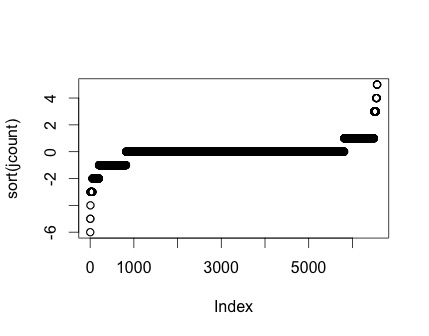
\includegraphics[scale=0.5]{Jump}
\centering
\end{figure}








\end{document}
